\providecommand{\main}{../../../..}
\documentclass[\main/dresen_thesis.tex]{subfiles}

\begin{document}
  \label{sec:monolayers:preparation:solventProperties}
  \begin{figure}[tb]
    \centering
    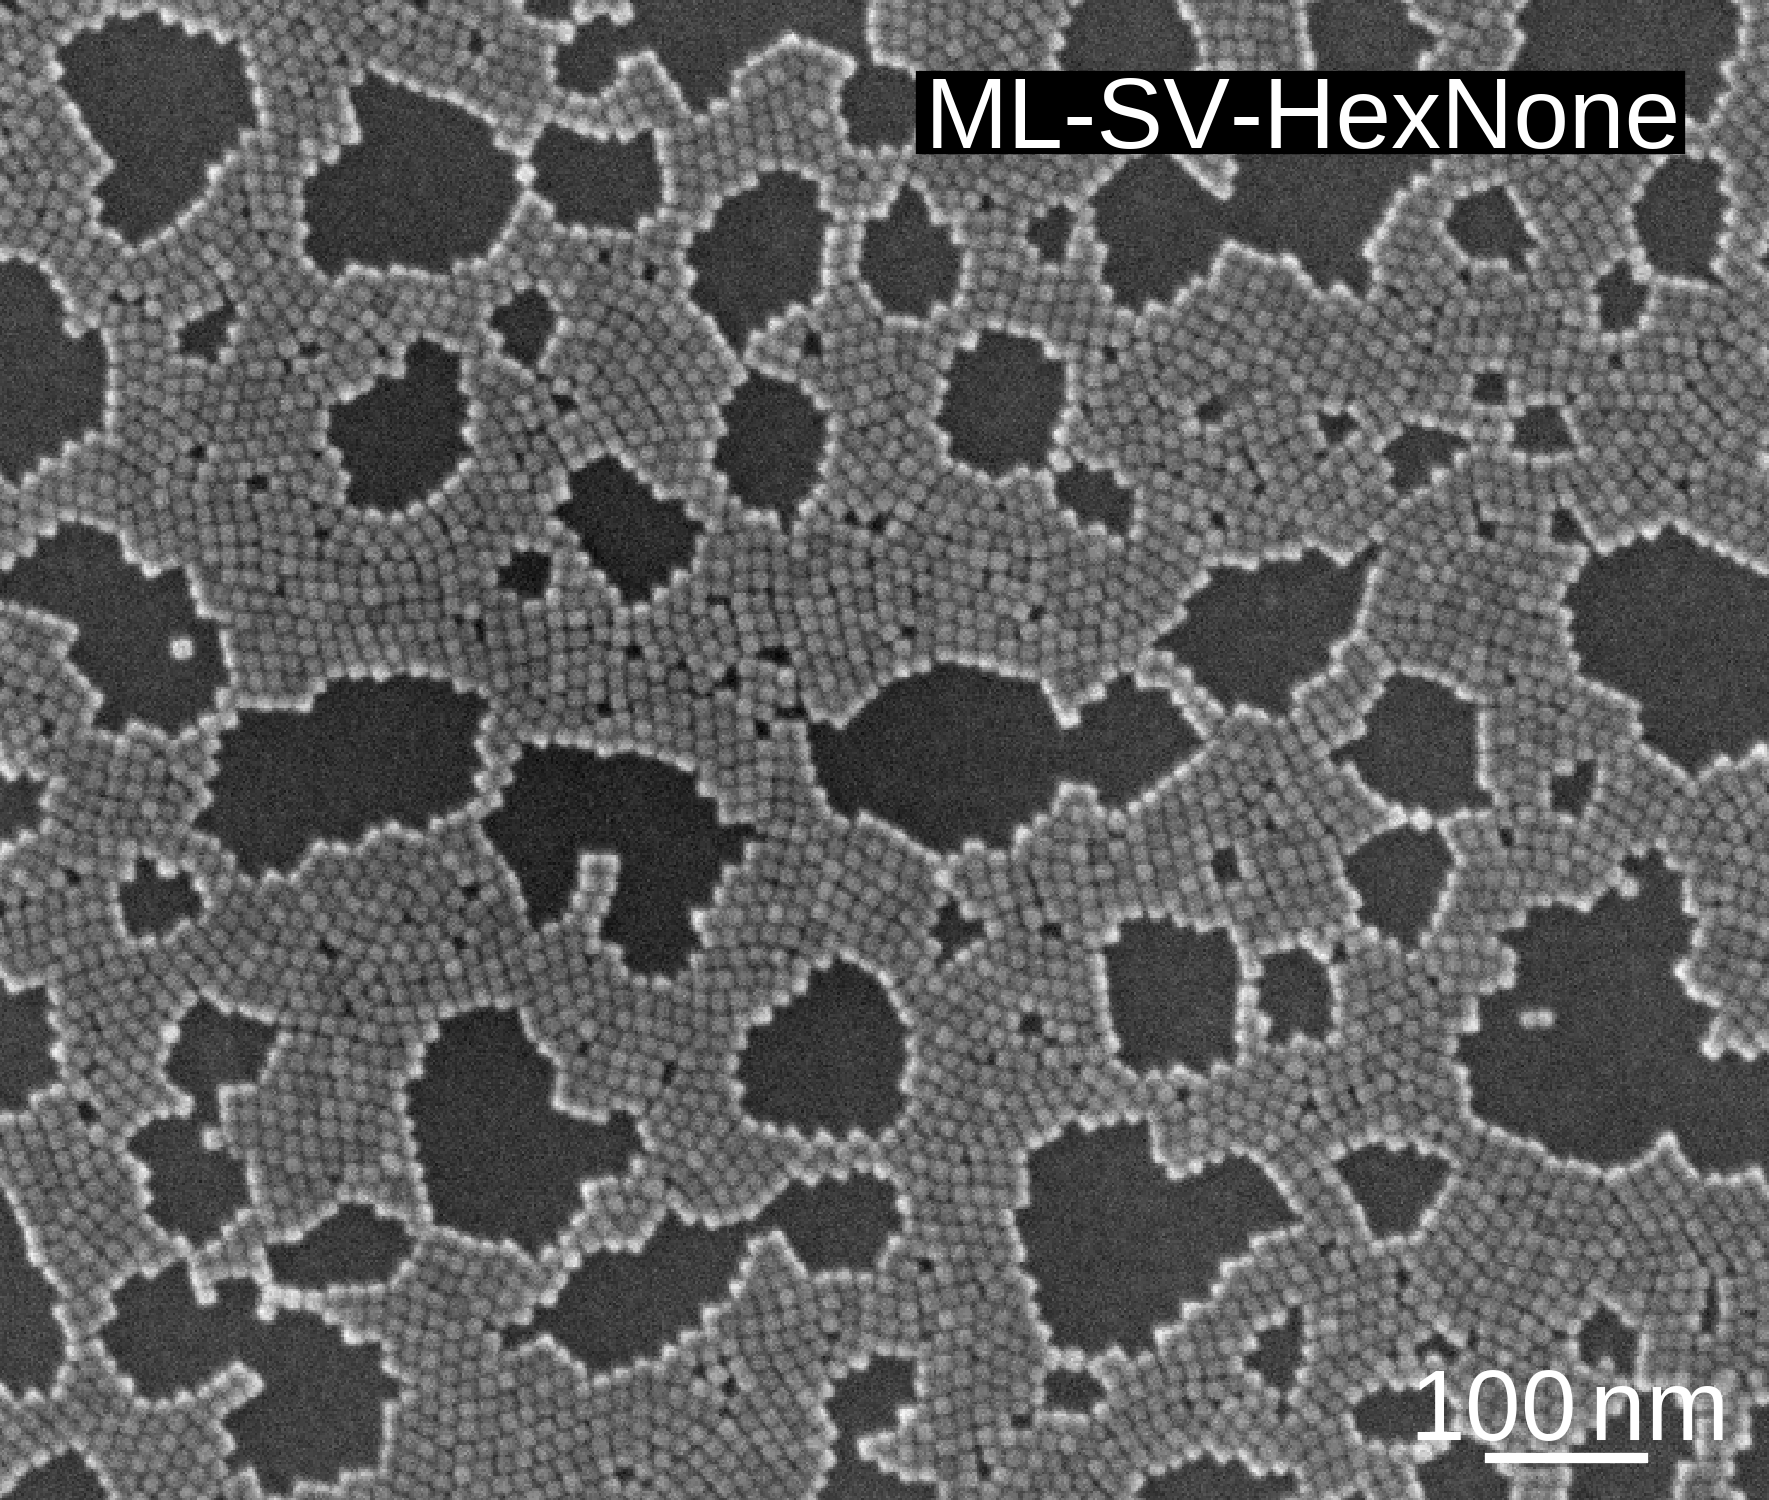
\includegraphics{monolayers_SEM_ML-SV-HexNone}
    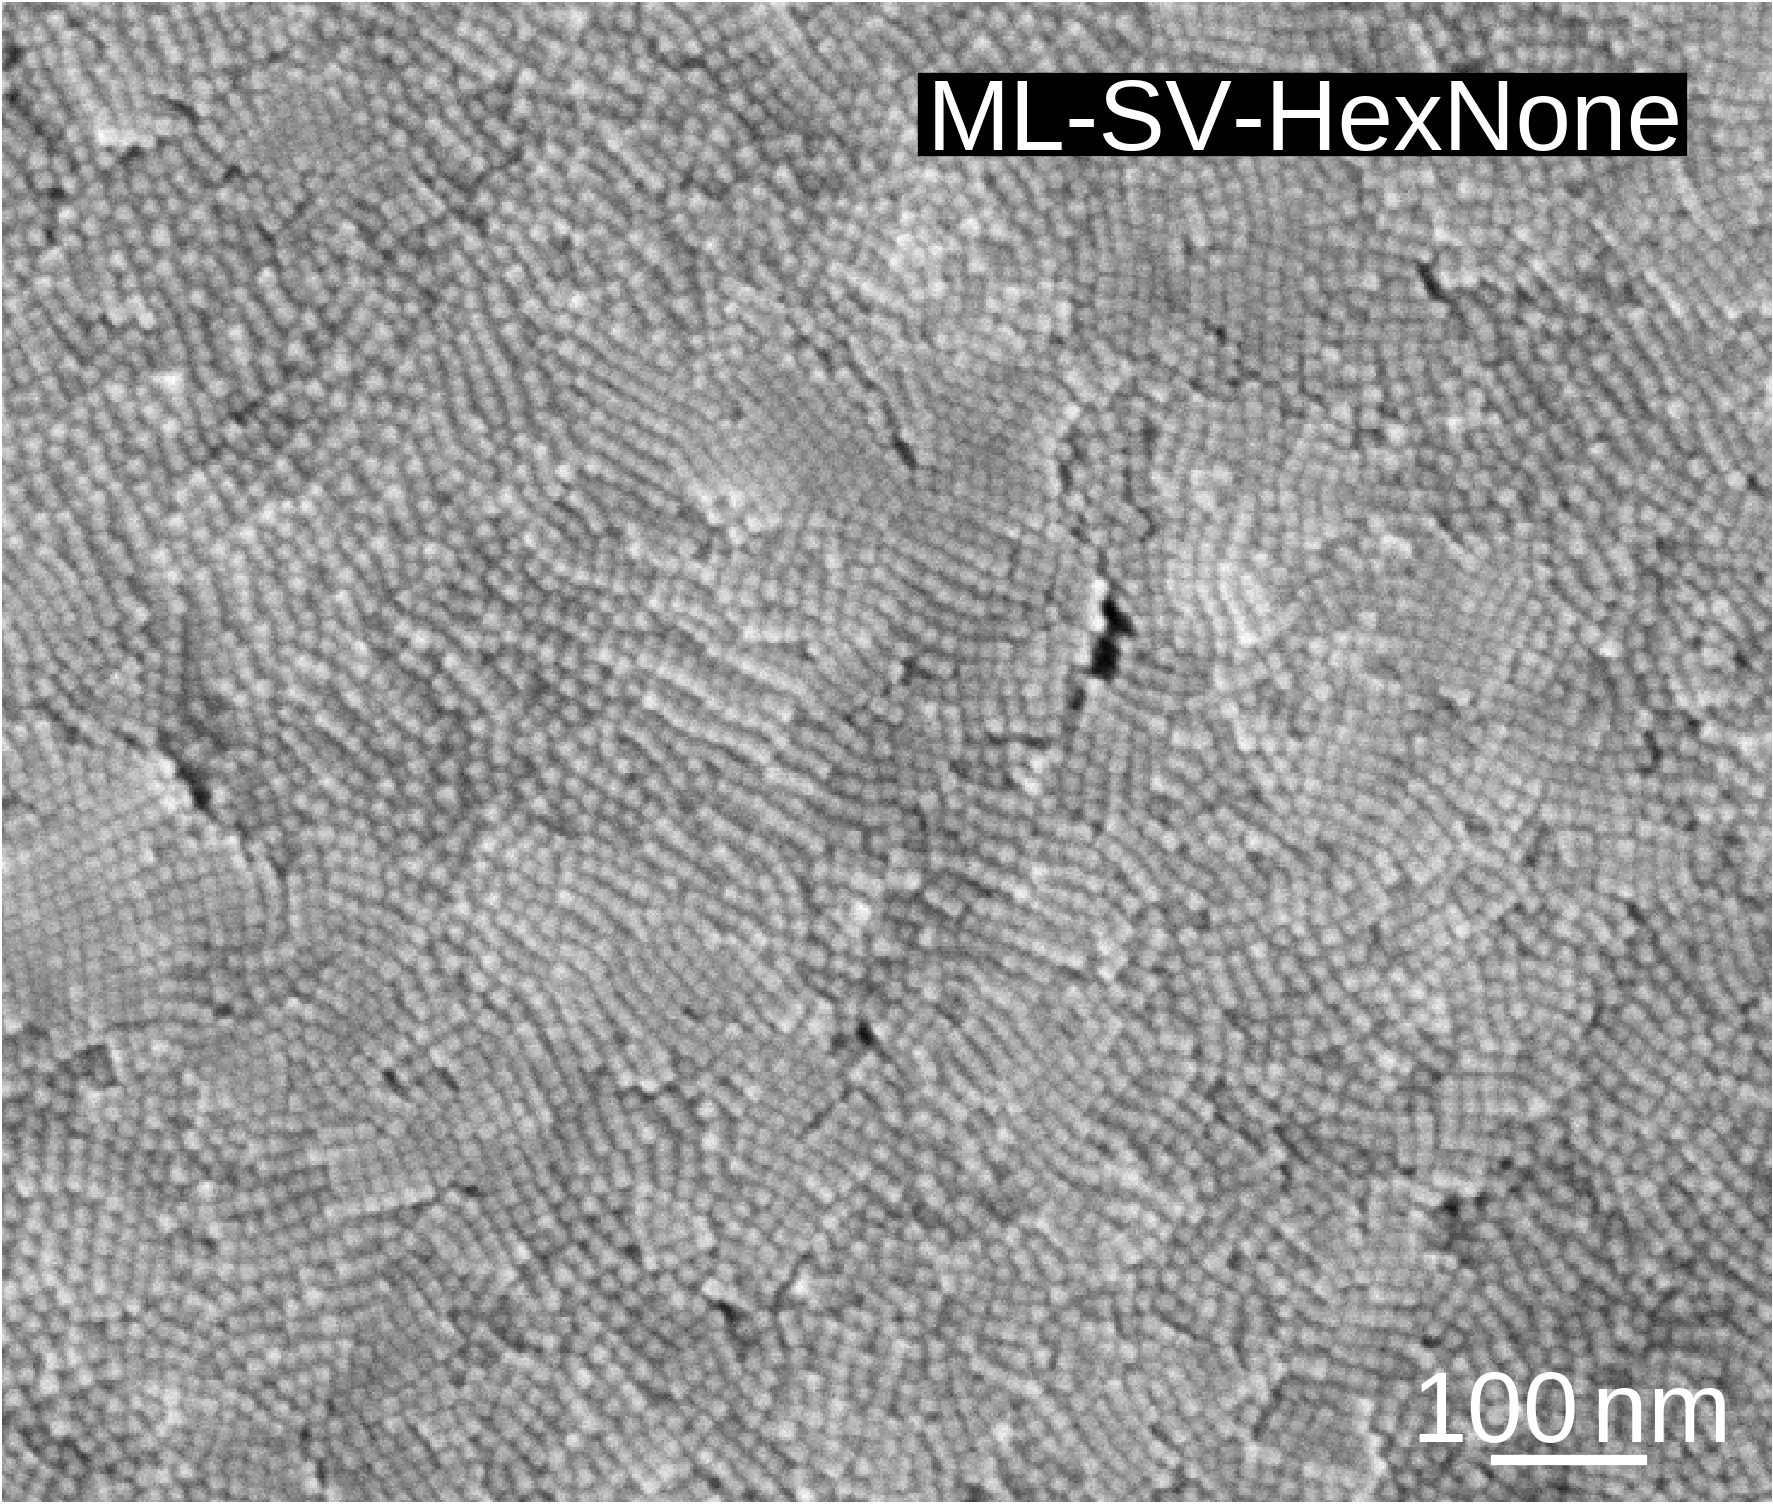
\includegraphics{monolayers_SEM_ML-SV-HexNone2}
    \caption{\label{fig:monolayers:preparation:solventVariation:semNoCoSolvent}SEM micrograph of Ol-CoFe-C nanoparticles after drop casting from $\mathit{n}$-hexane and without a co-solvent addend from two different positions on the same substrate.}
  \end{figure}
  The solvent and co-solvent of the dispersion for the drop casting experiment determine the mobility of the nanoparticles and the time scales for a drop casting experiment.
  When oleic acid ligated nanocubes are drop casted as-prepared at low concentration from an organic dispersion such as n-hexane without any additional addends or setups, no long-range order is observed and the overall sample quality is inhomogeneous as seen in \reffig{fig:monolayers:preparation:solventVariation:semNoCoSolvent}.
  On different positions of the substrate, the nanoparticles have either connected with many holes in between or they are heaped in a bulk, showing in both cases only short-range order.
  The micrographs suggest sub-optimal wetting conditions for the solvent and a missing mechanism in the self-assembly process for an even distribution of the particles across the substrate.

  \subsubsection{Variation of Alkanes / Alkenes as Solvent / Co-Solvent}
    To study the effect of the solvent choice on the structural long-range order for drop casted nanocubes, a series of  primary/co-solvent mixtures are studied by performing drop casting experiments with the nanocubes Ol-CoFe-C.
    In the following four combinations solvent/co-solvent combinations are discussed in detail: A sample of an alkene with a relatively low boiling point, 1-tetradecene, together with \textit{n}-hexane (ML-SV-HexTet), and three samples of 1-octadecene with varied alkanes \textit{n}-pentane (ML-SV-PenOct), \textit{n}-hexane (ML-SV-HexOct) and \textit{n}-heptane (ML-SV-HepOct).

    \begin{figure}[tb]
      \centering
      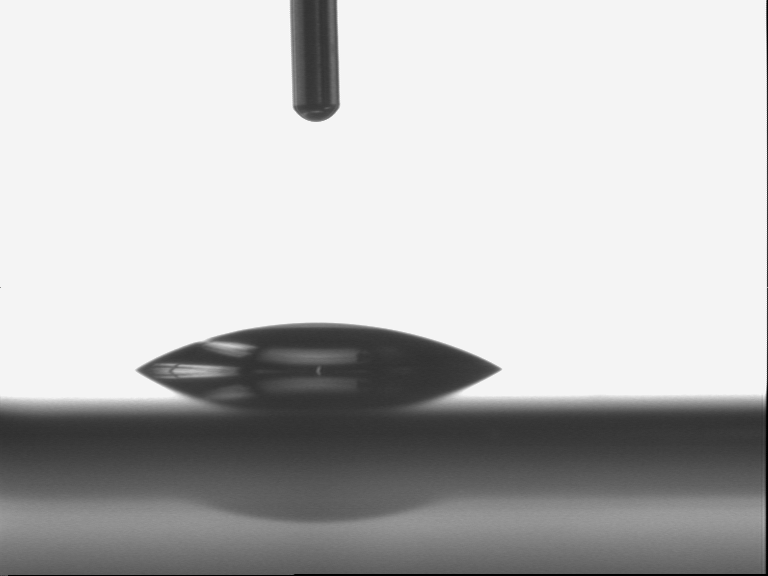
\includegraphics[width=0.31\textwidth]{monolayer_contactAngle_Water}
      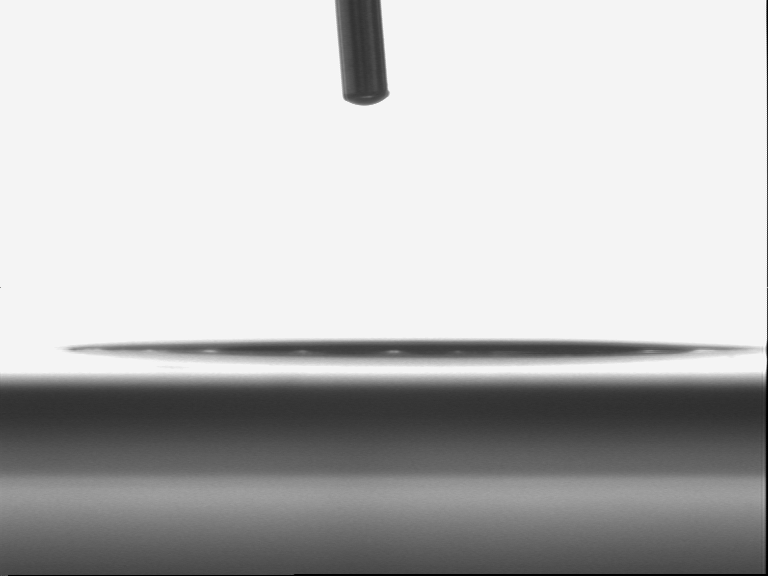
\includegraphics[width=0.31\textwidth]{monolayer_contactAngle_OlCoFeC}
      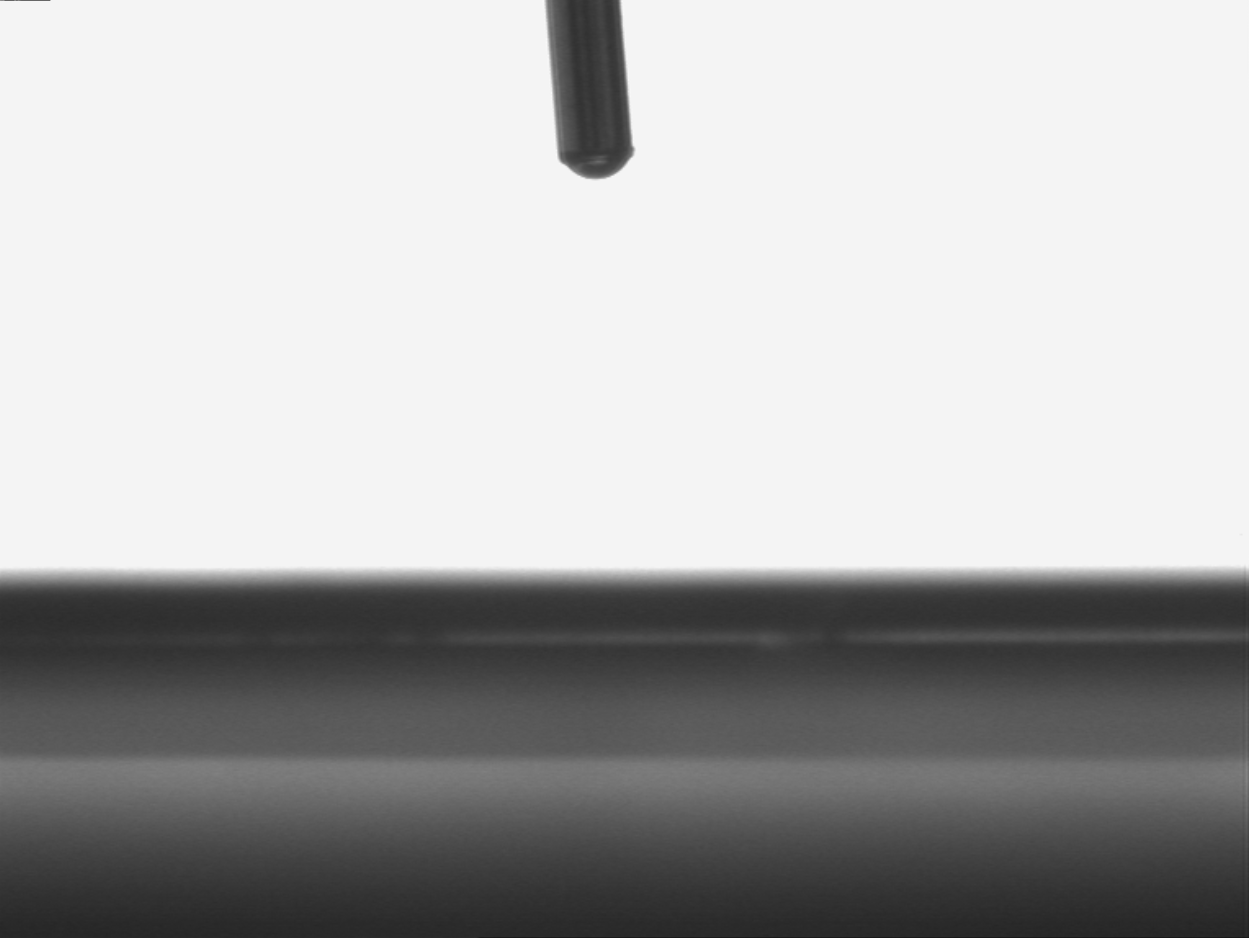
\includegraphics[width=0.31\textwidth]{monolayer_contactAngle_OlCoFeCOctadecene2Percent}
      \caption{\label{fig:monolayers:preparation:contactAngle}Side-view camera image of a droplet of water (left), a droplet of $\mathit{n}$-hexane (center) and a droplet of $\mathit{n}$-hexane with $2 \unit{\%}$ 1-octadecene (right) on a silicon substrate.}
    \end{figure}
    An effect of the co-solvent addend that is immediately visible during the drop casting procedure is the improved spreading of the dispersion on the substrate.
    Attempts to measure the contact angle between dispersion and silicon substrate are shown in \reffig{fig:monolayers:preparation:contactAngle} in comparison to a droplet of water on silicon.
    While the contact angle of $\mathit{n}$-hexane is $<10^\circ$ on silicon, the addition of a small amount of octadecene as addend makes the droplet no longer visible in a side view meaning that it evenly spreads on the surface.
    From which it can be seen that the alkene addend greatly increases the wetting properties of the dispersion.

    \begin{figure}[tb]
      \centering
      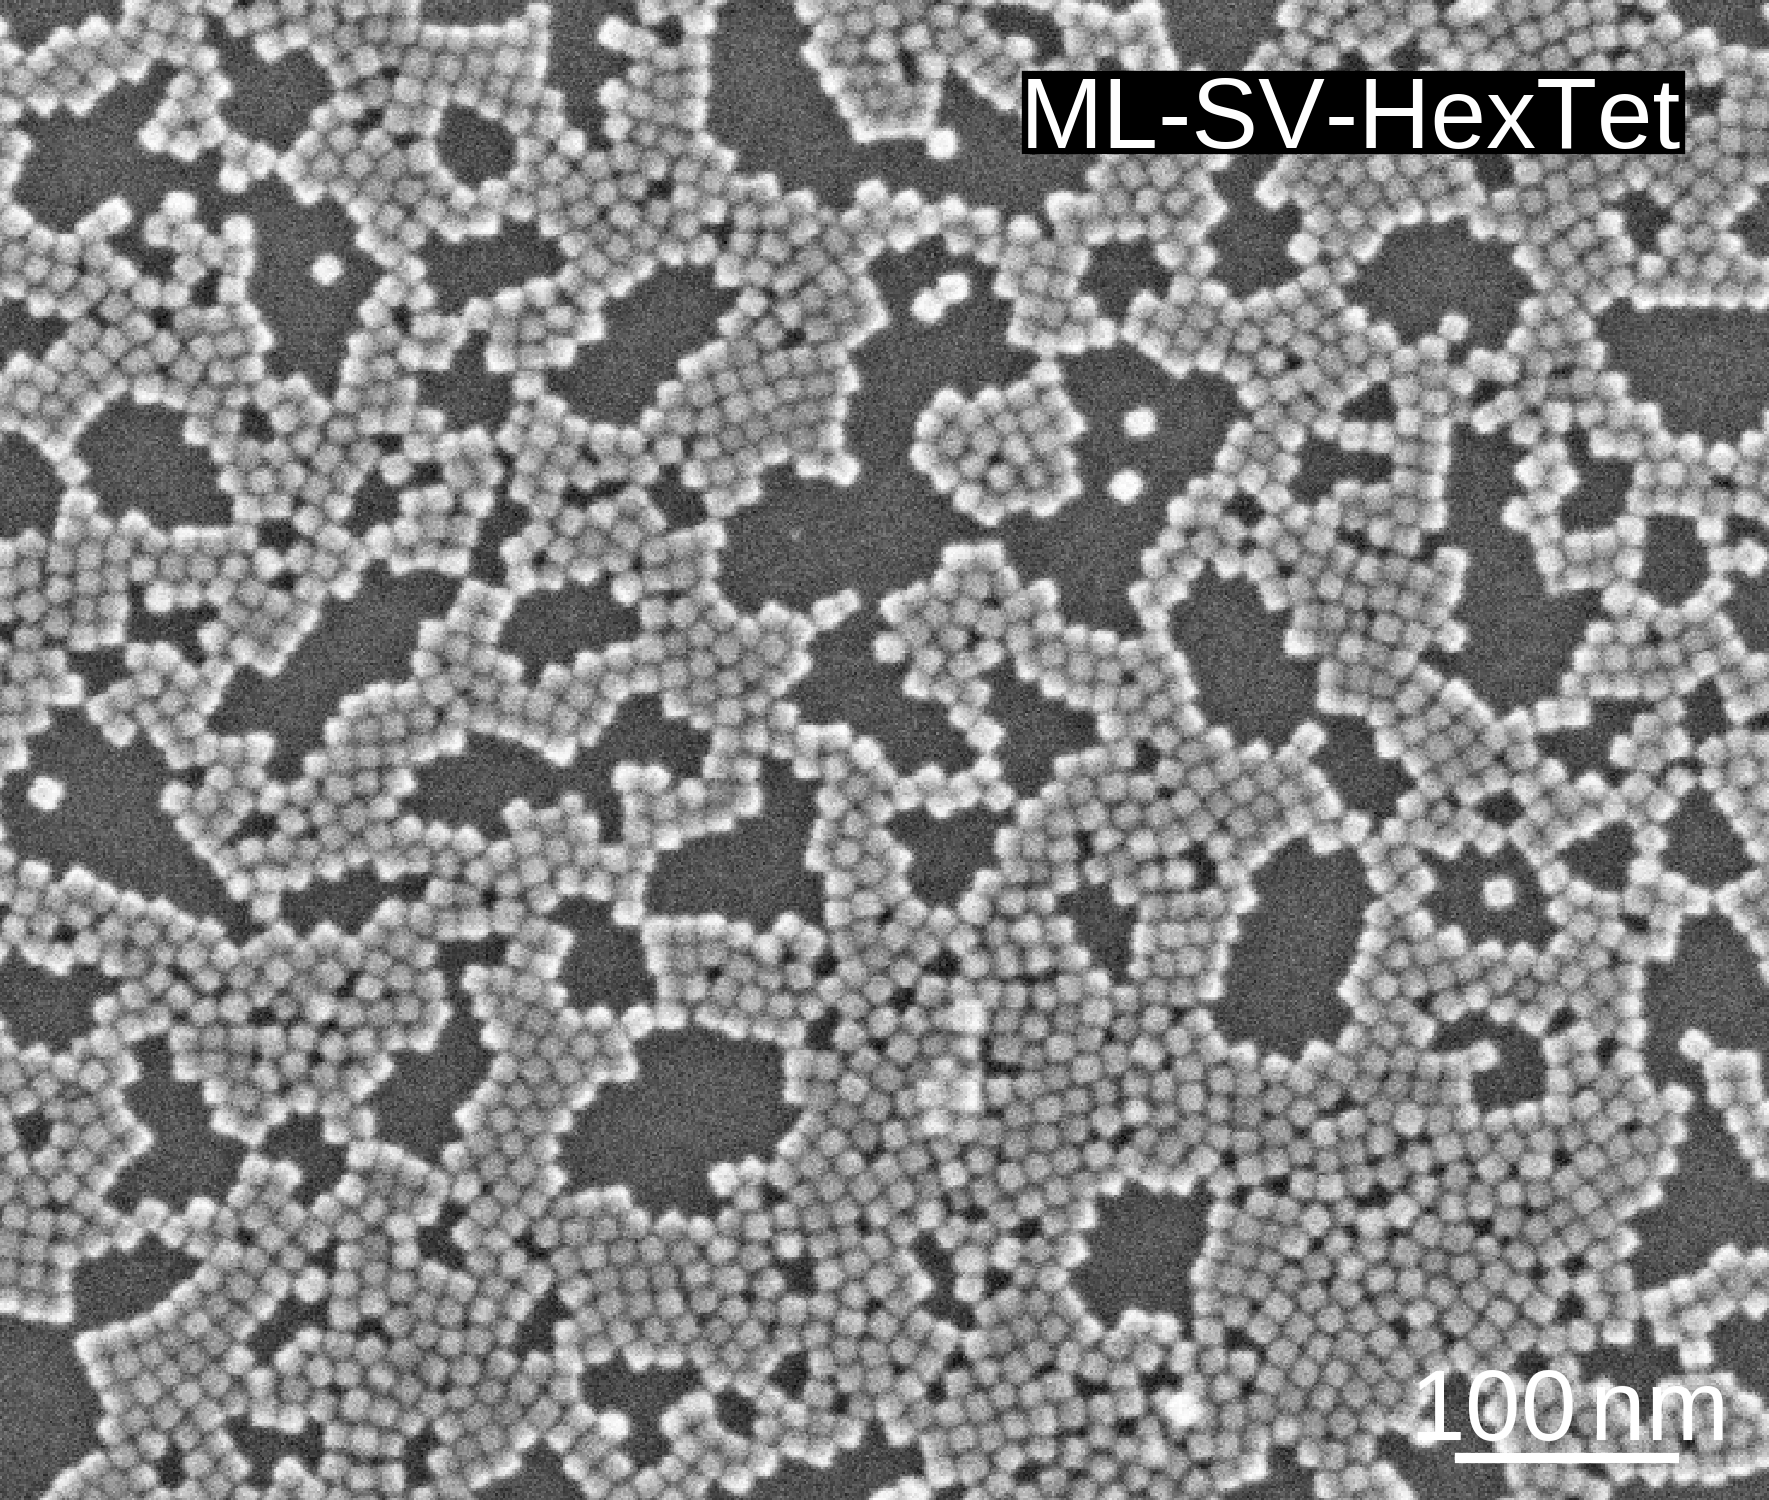
\includegraphics{monolayers_SEM_ML-SV-HexTet}
      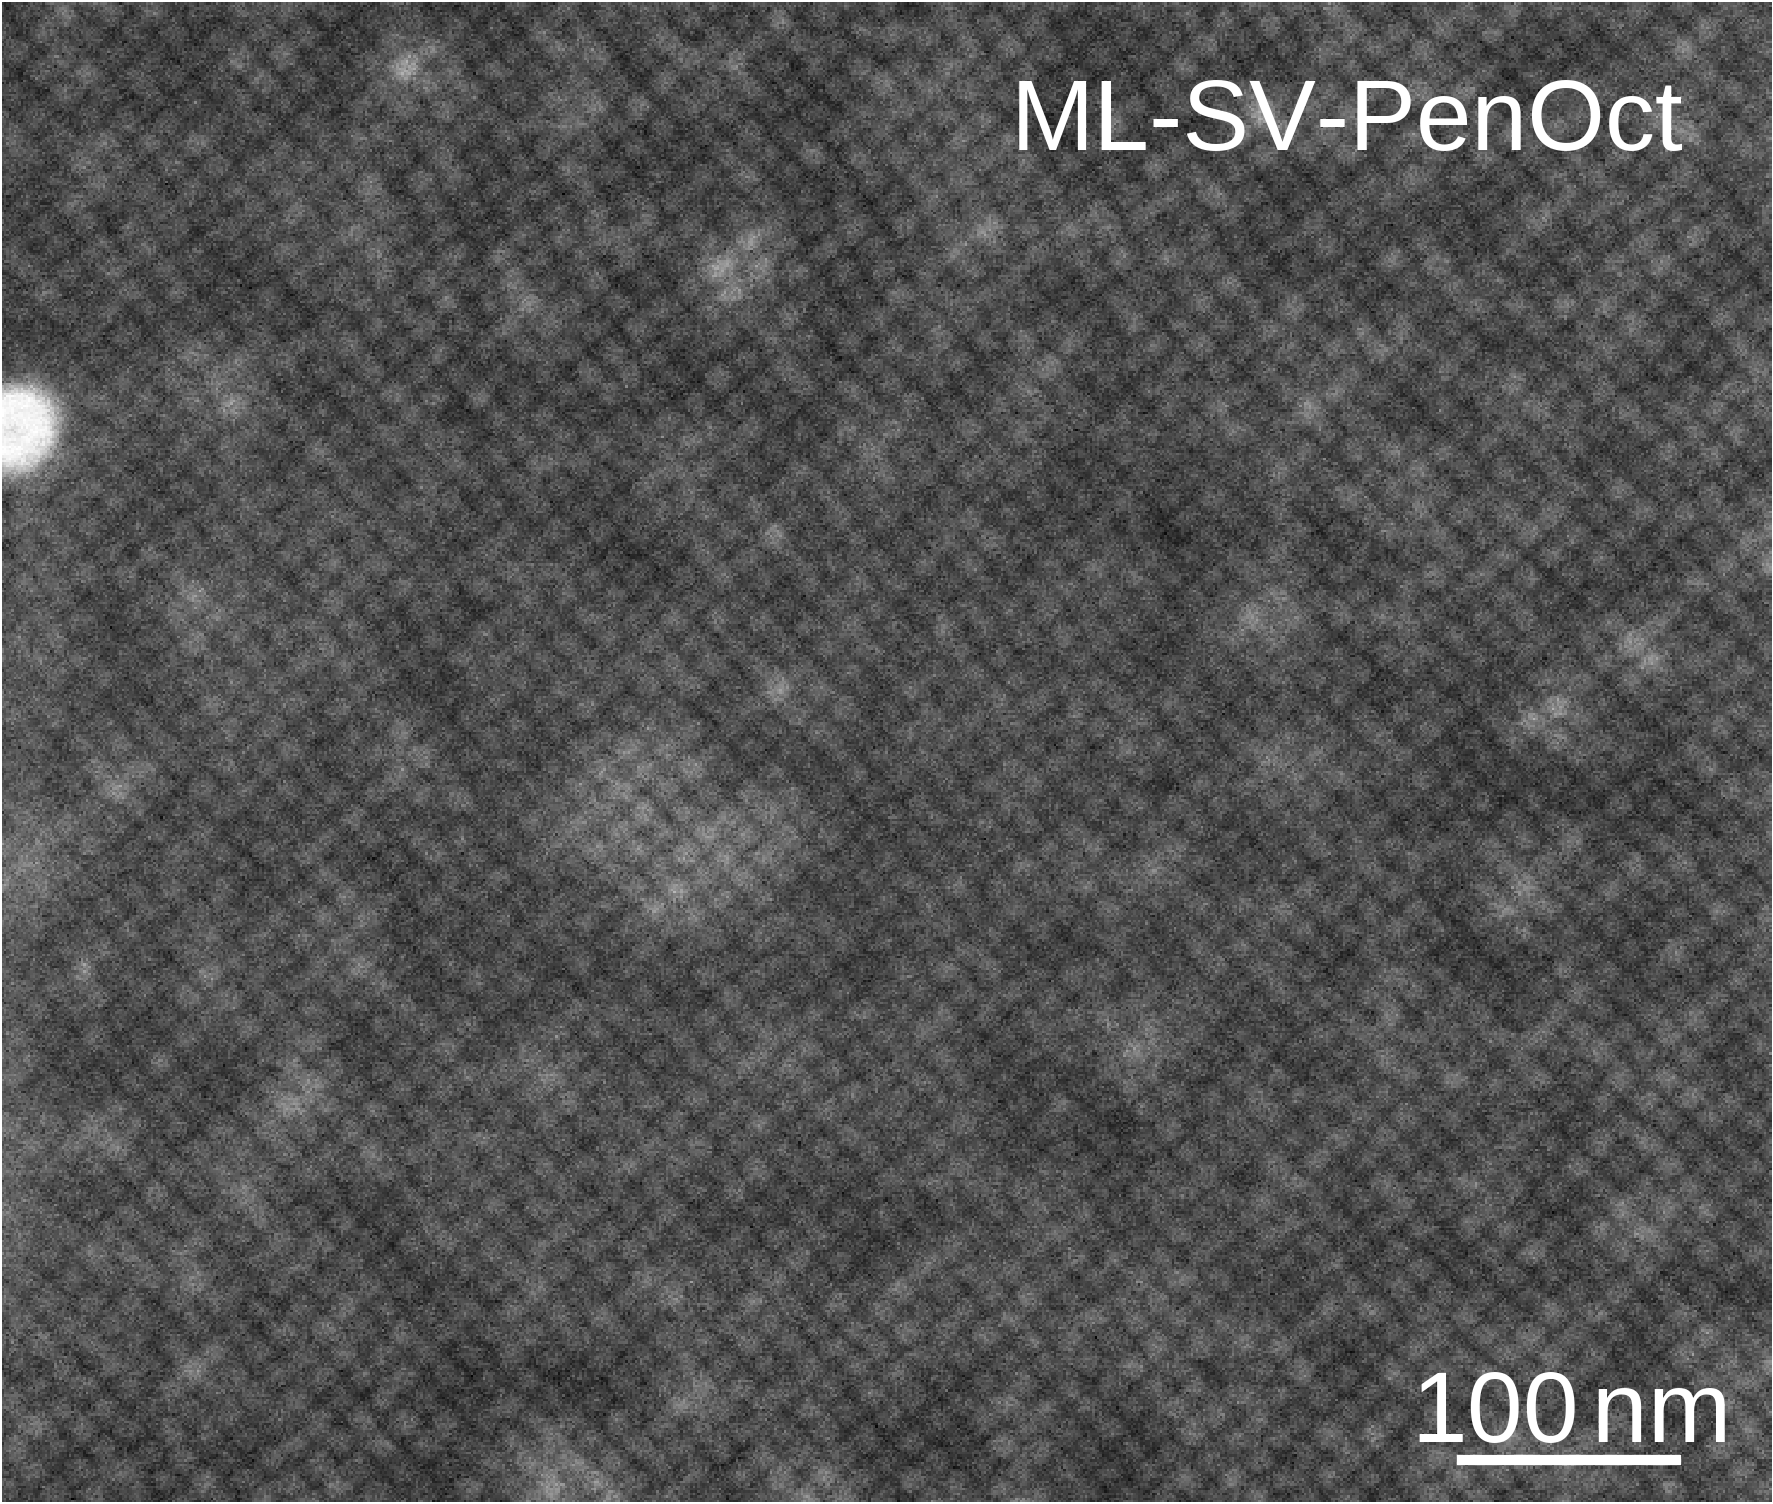
\includegraphics{monolayers_SEM_ML-SV-PenOct}
      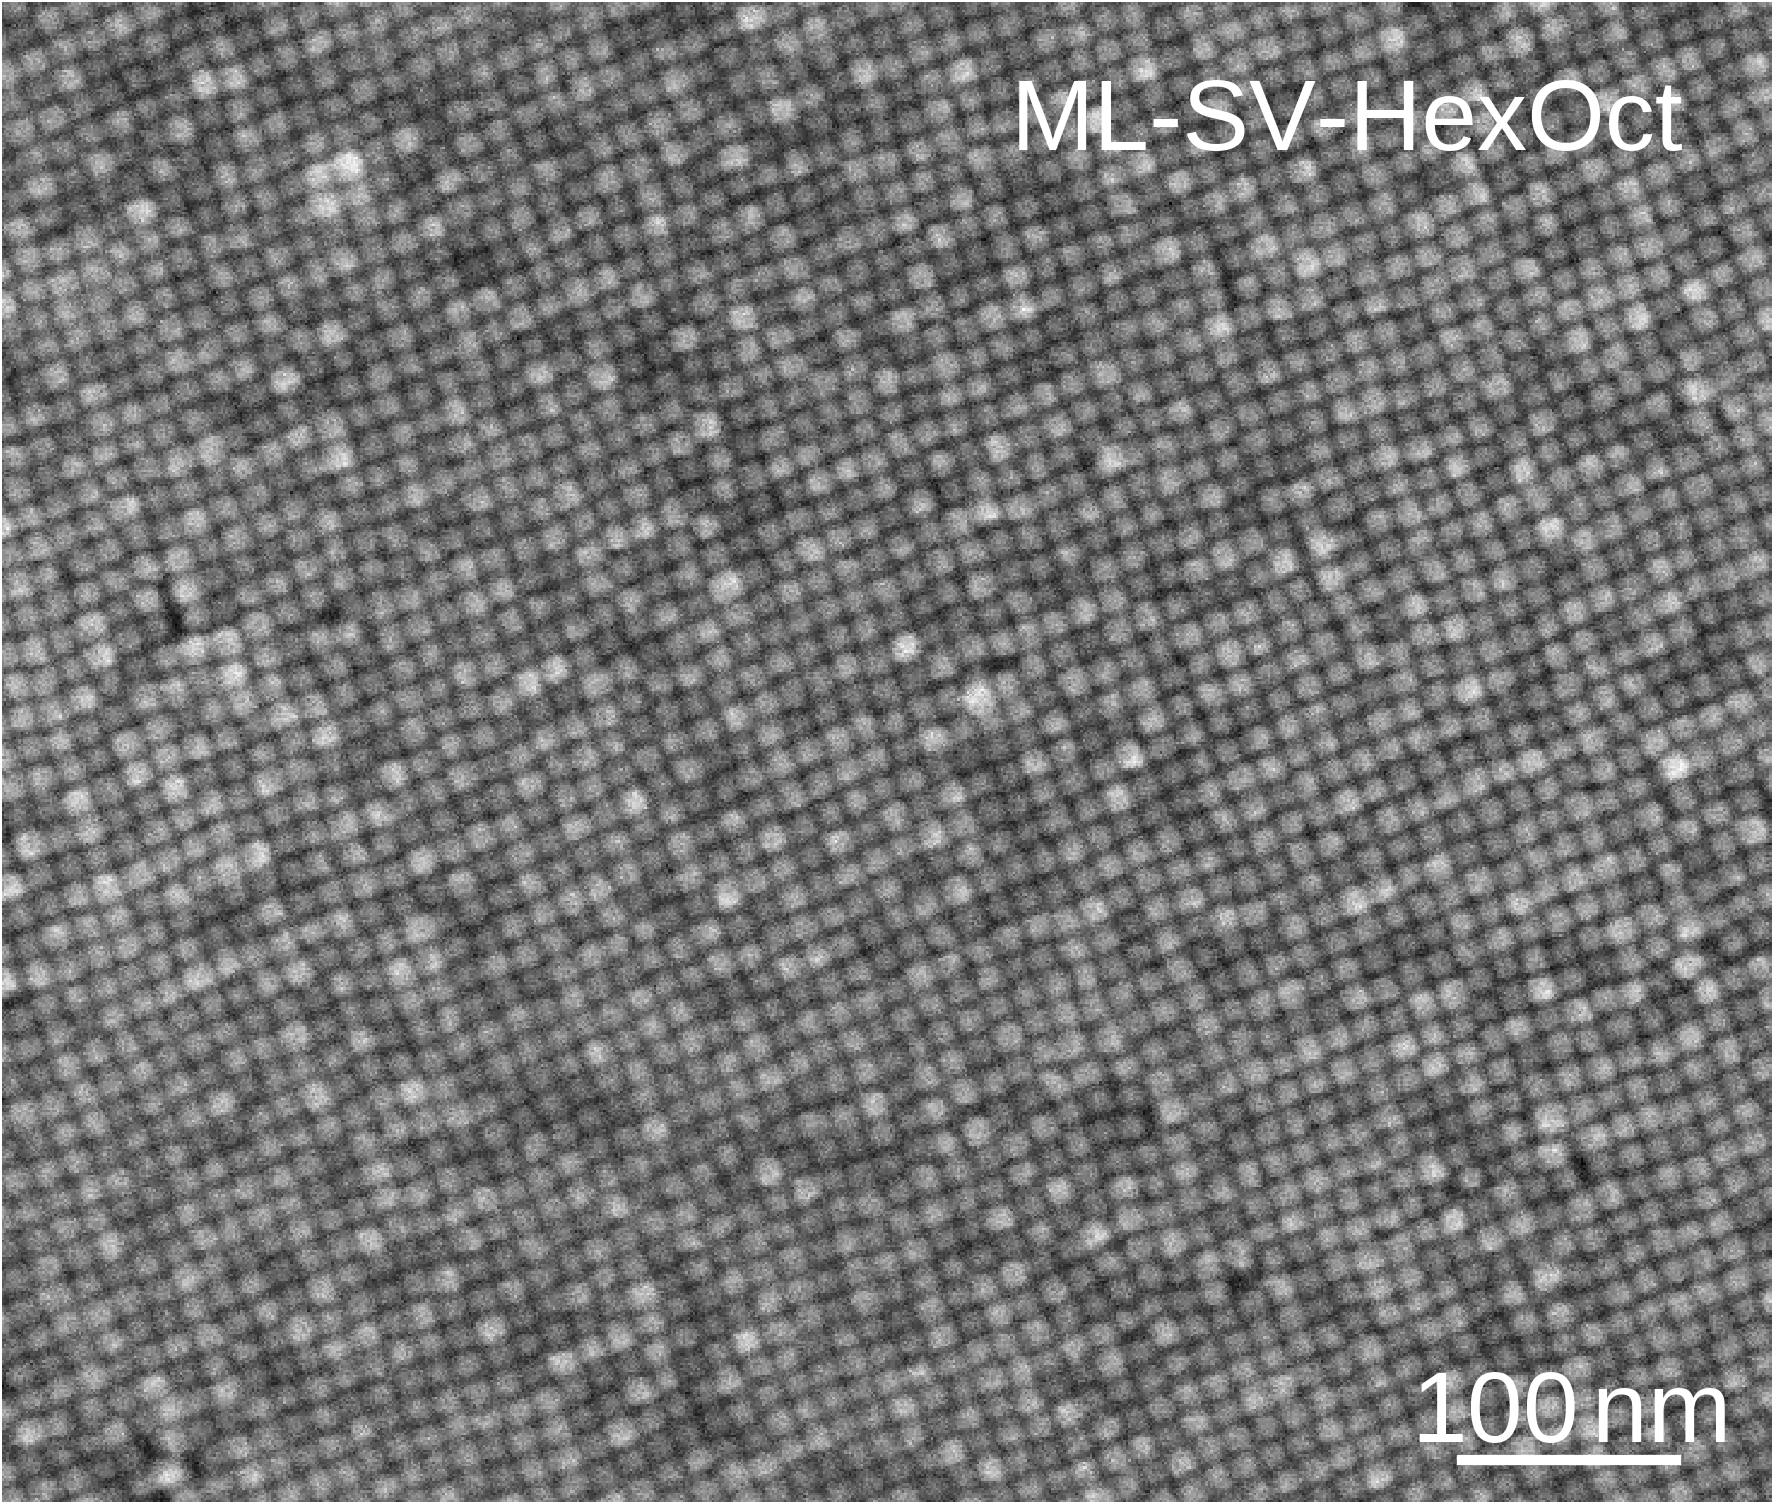
\includegraphics{monolayers_SEM_ML-SV-HexOct}
      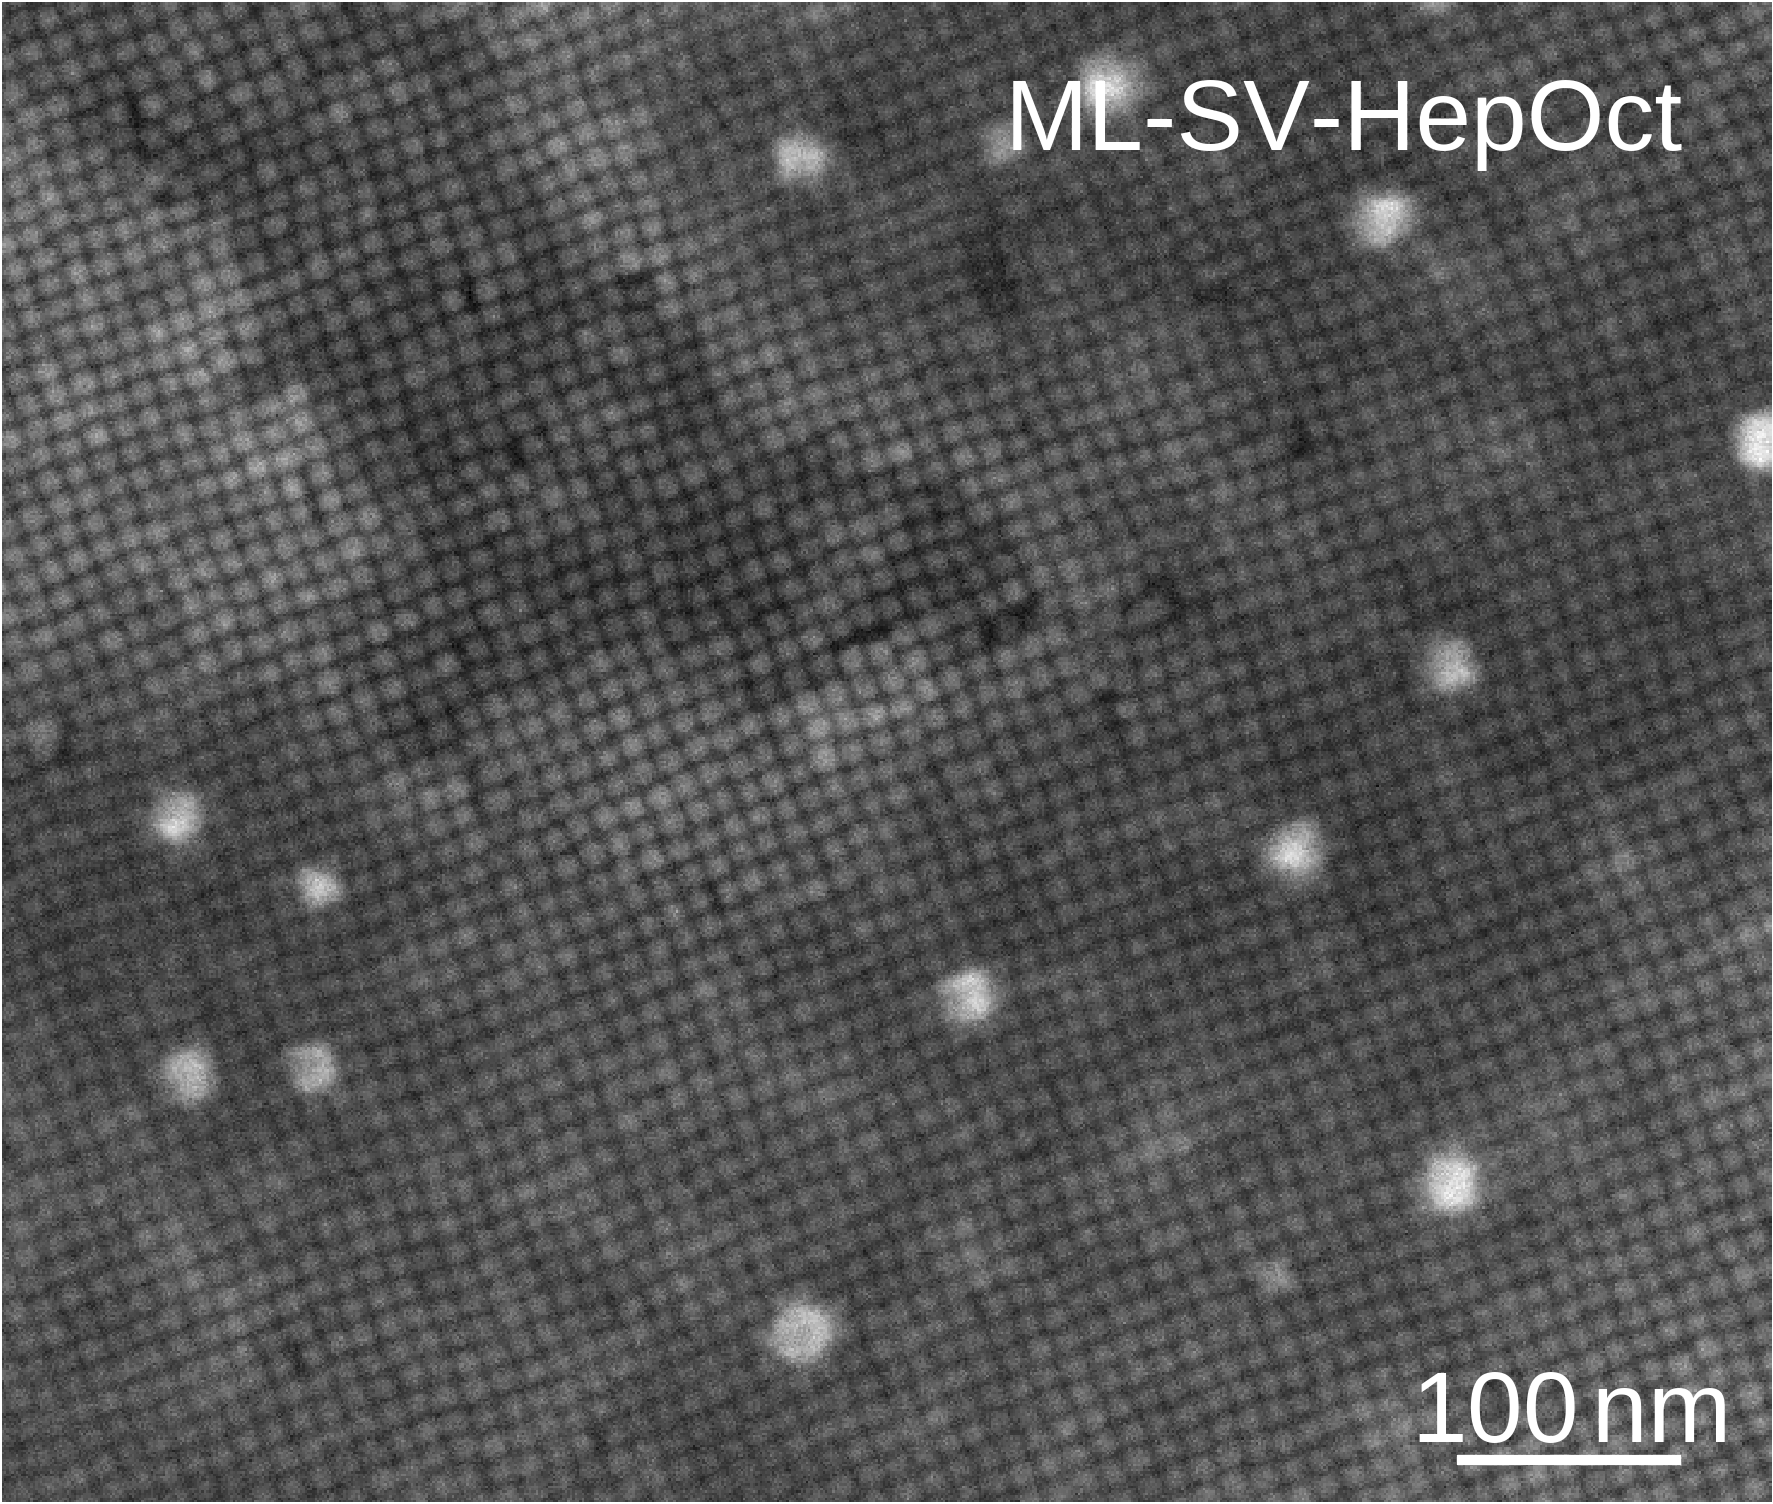
\includegraphics{monolayers_SEM_ML-SV-HepOct}
      \caption{\label{fig:monolayers:preparation:solventVariation:sem}Scanning electron microscopy of Ol-CoFe-C nanoparticles after drop casting using $\mathit{n}$-hexane/tetradecene (upper left), $\mathit{n}$-pentane/octadecene (upper right), $\mathit{n}$-hexane/octadecene (lower left) and $\mathit{n}$-heptane/octadecene (lower right) as solvents.}
    \end{figure}
    In \reffig{fig:monolayers:preparation:solventVariation:sem} SEM micrographs of the four drop casted solvent/co-solvent combinations are shown.
    A result that is imminently visible is that an alkene with a relatively low boiling point leads to no order formation, whereas  combinations with 1-octadecene show for all alkanes local square order formation.

    Additionally visible on the micrographs of ML-SV-PenOct and ML-SV-HepOct are small bright spots on top of the ordered nanoparticles.
    Closer inspection of the spots by using the scanning electron microscope show that these spots can be melted with the electron beam.
    As the substrate have been baked for several hours at elevated temperatures of $140 \unit{^\circ C}$ prior the measurement and as the SEM has a ultra-high vacuum during the measurements, these dissolvable organic compounds must have a high vapor pressure to resist removal.
    It can therefore be assumed with high certainty that the bright spots are remnants of either octadecene or oleic acid.


    \begin{figure}[tb]
      \centering
      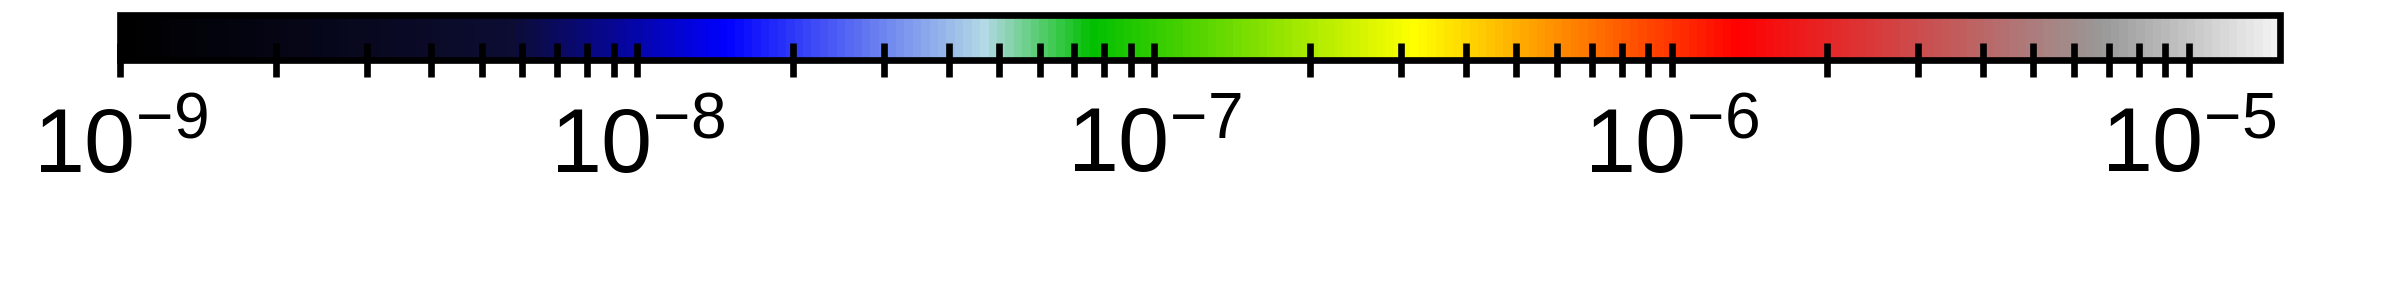
\includegraphics{monolayers_GISAXS_SVcbar}
      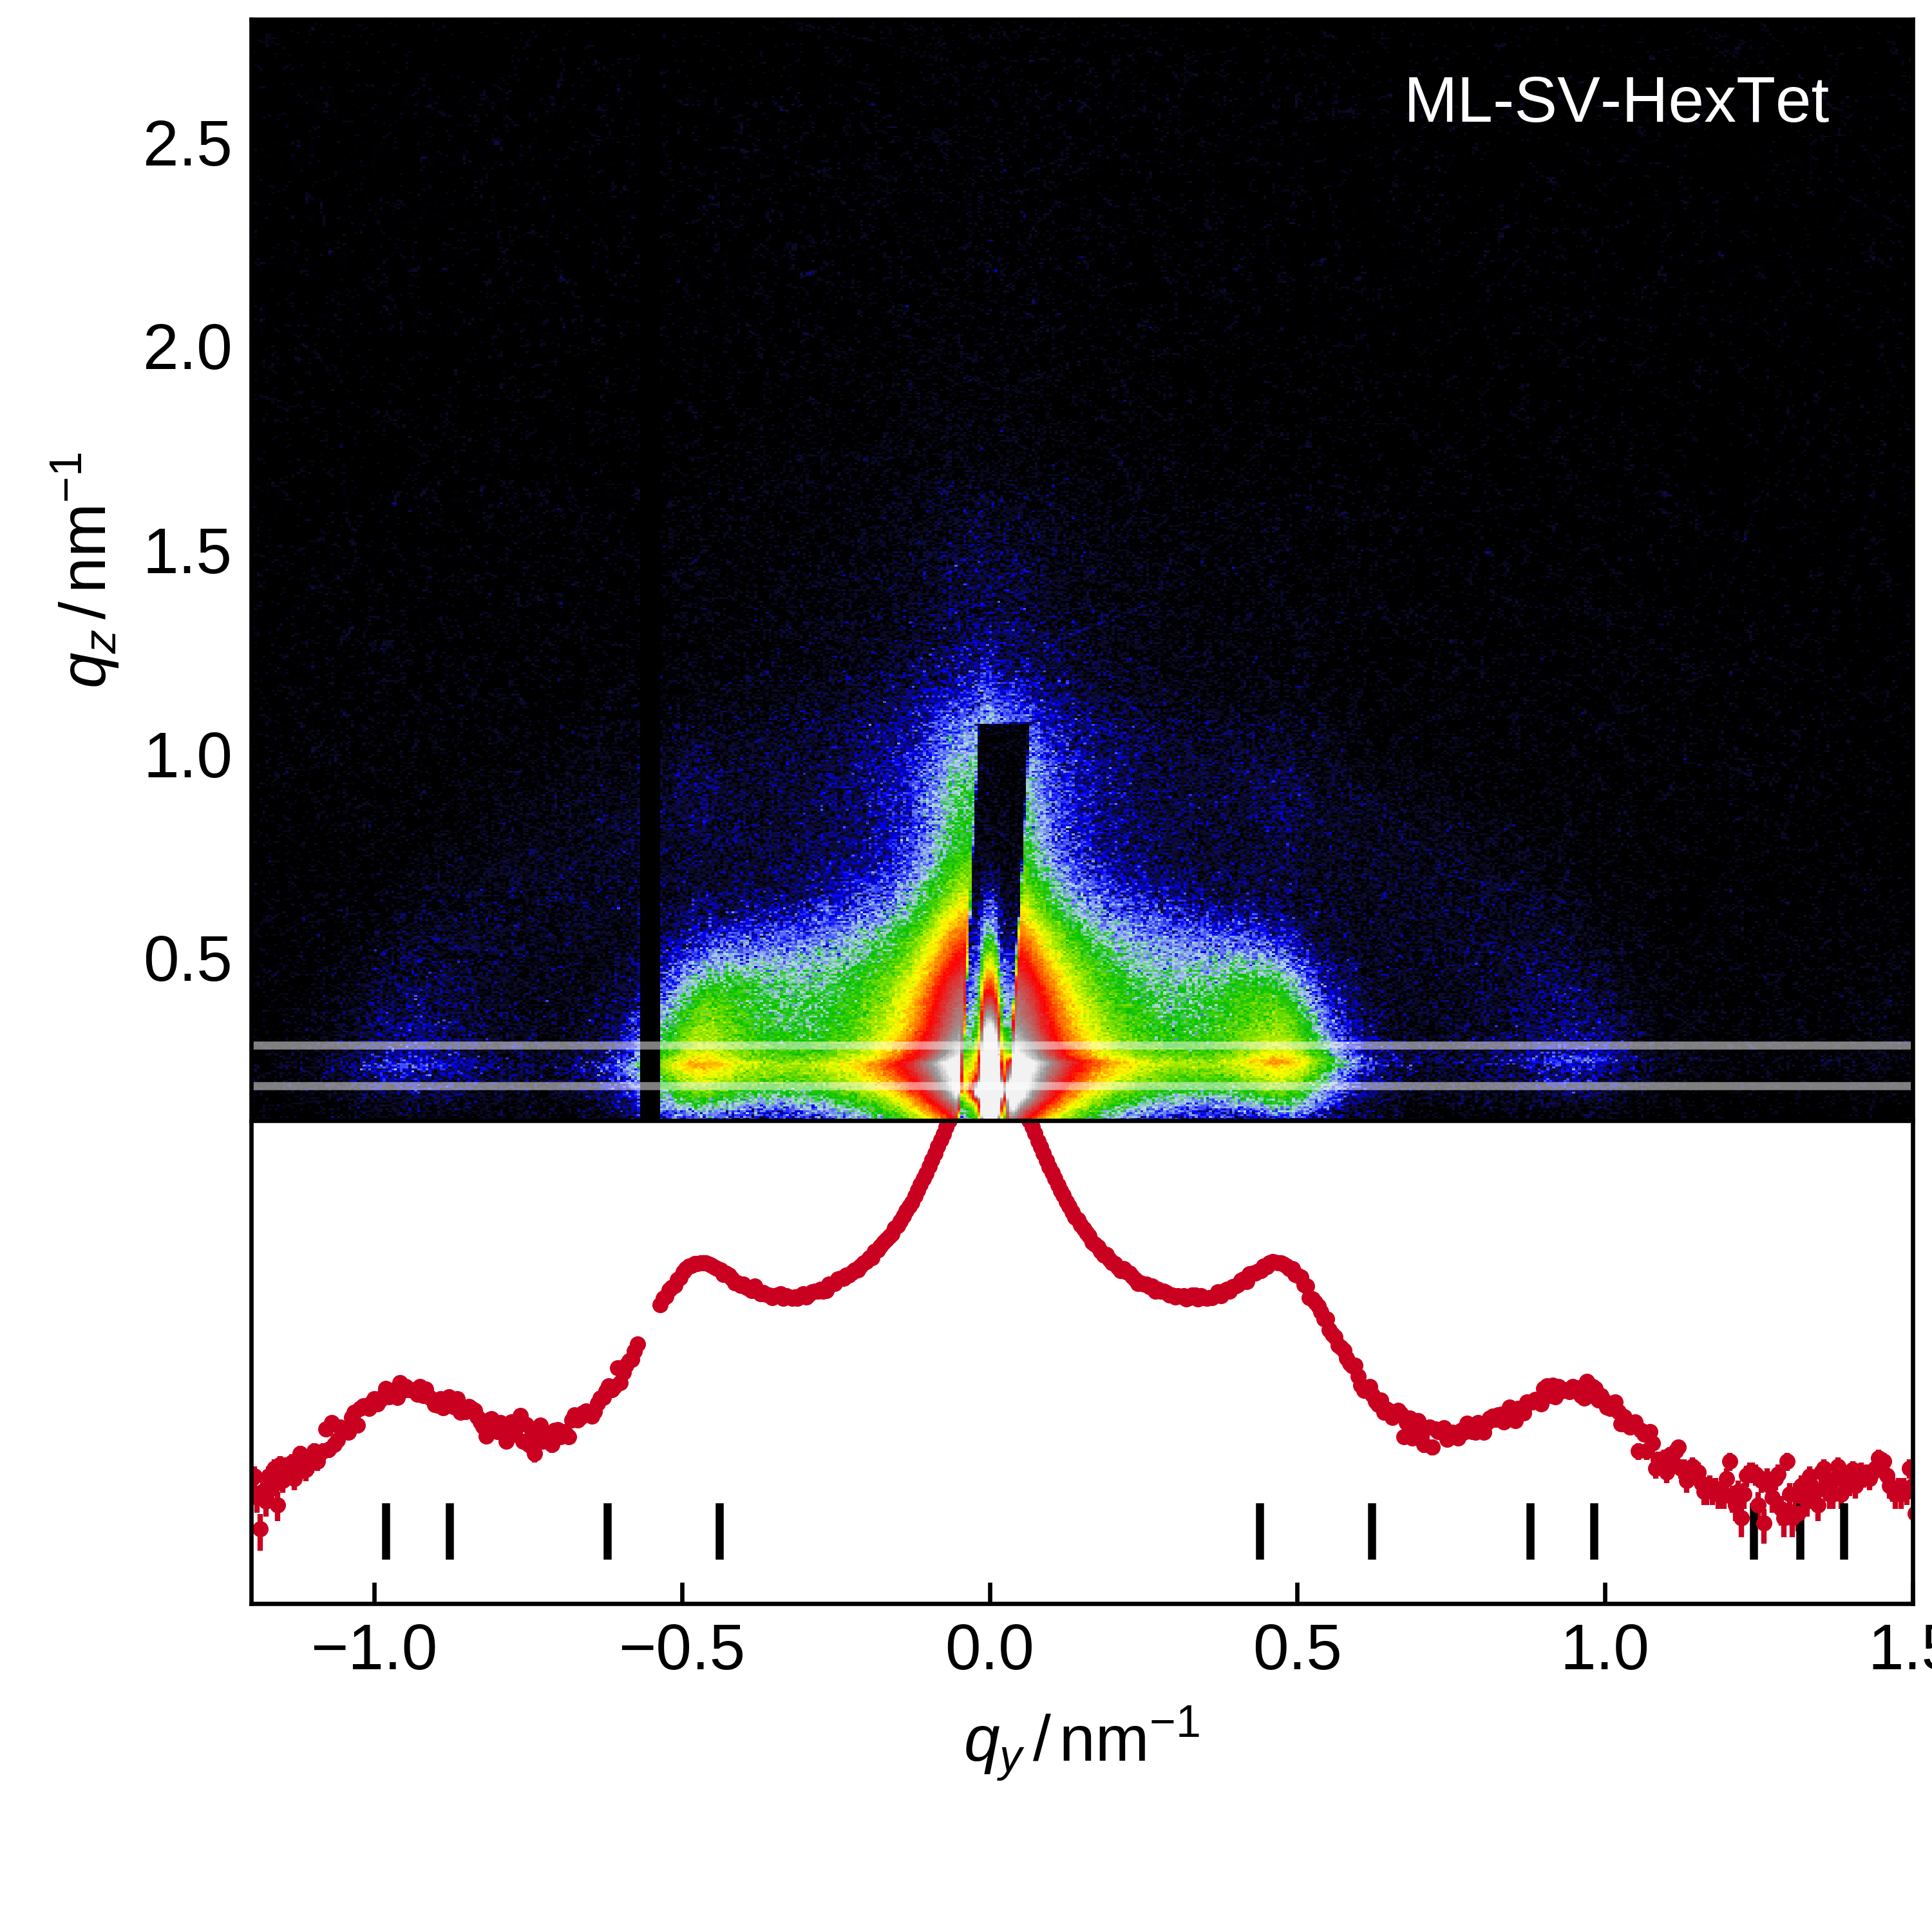
\includegraphics{monolayers_GISAXS_ML-SV-HexTet}
      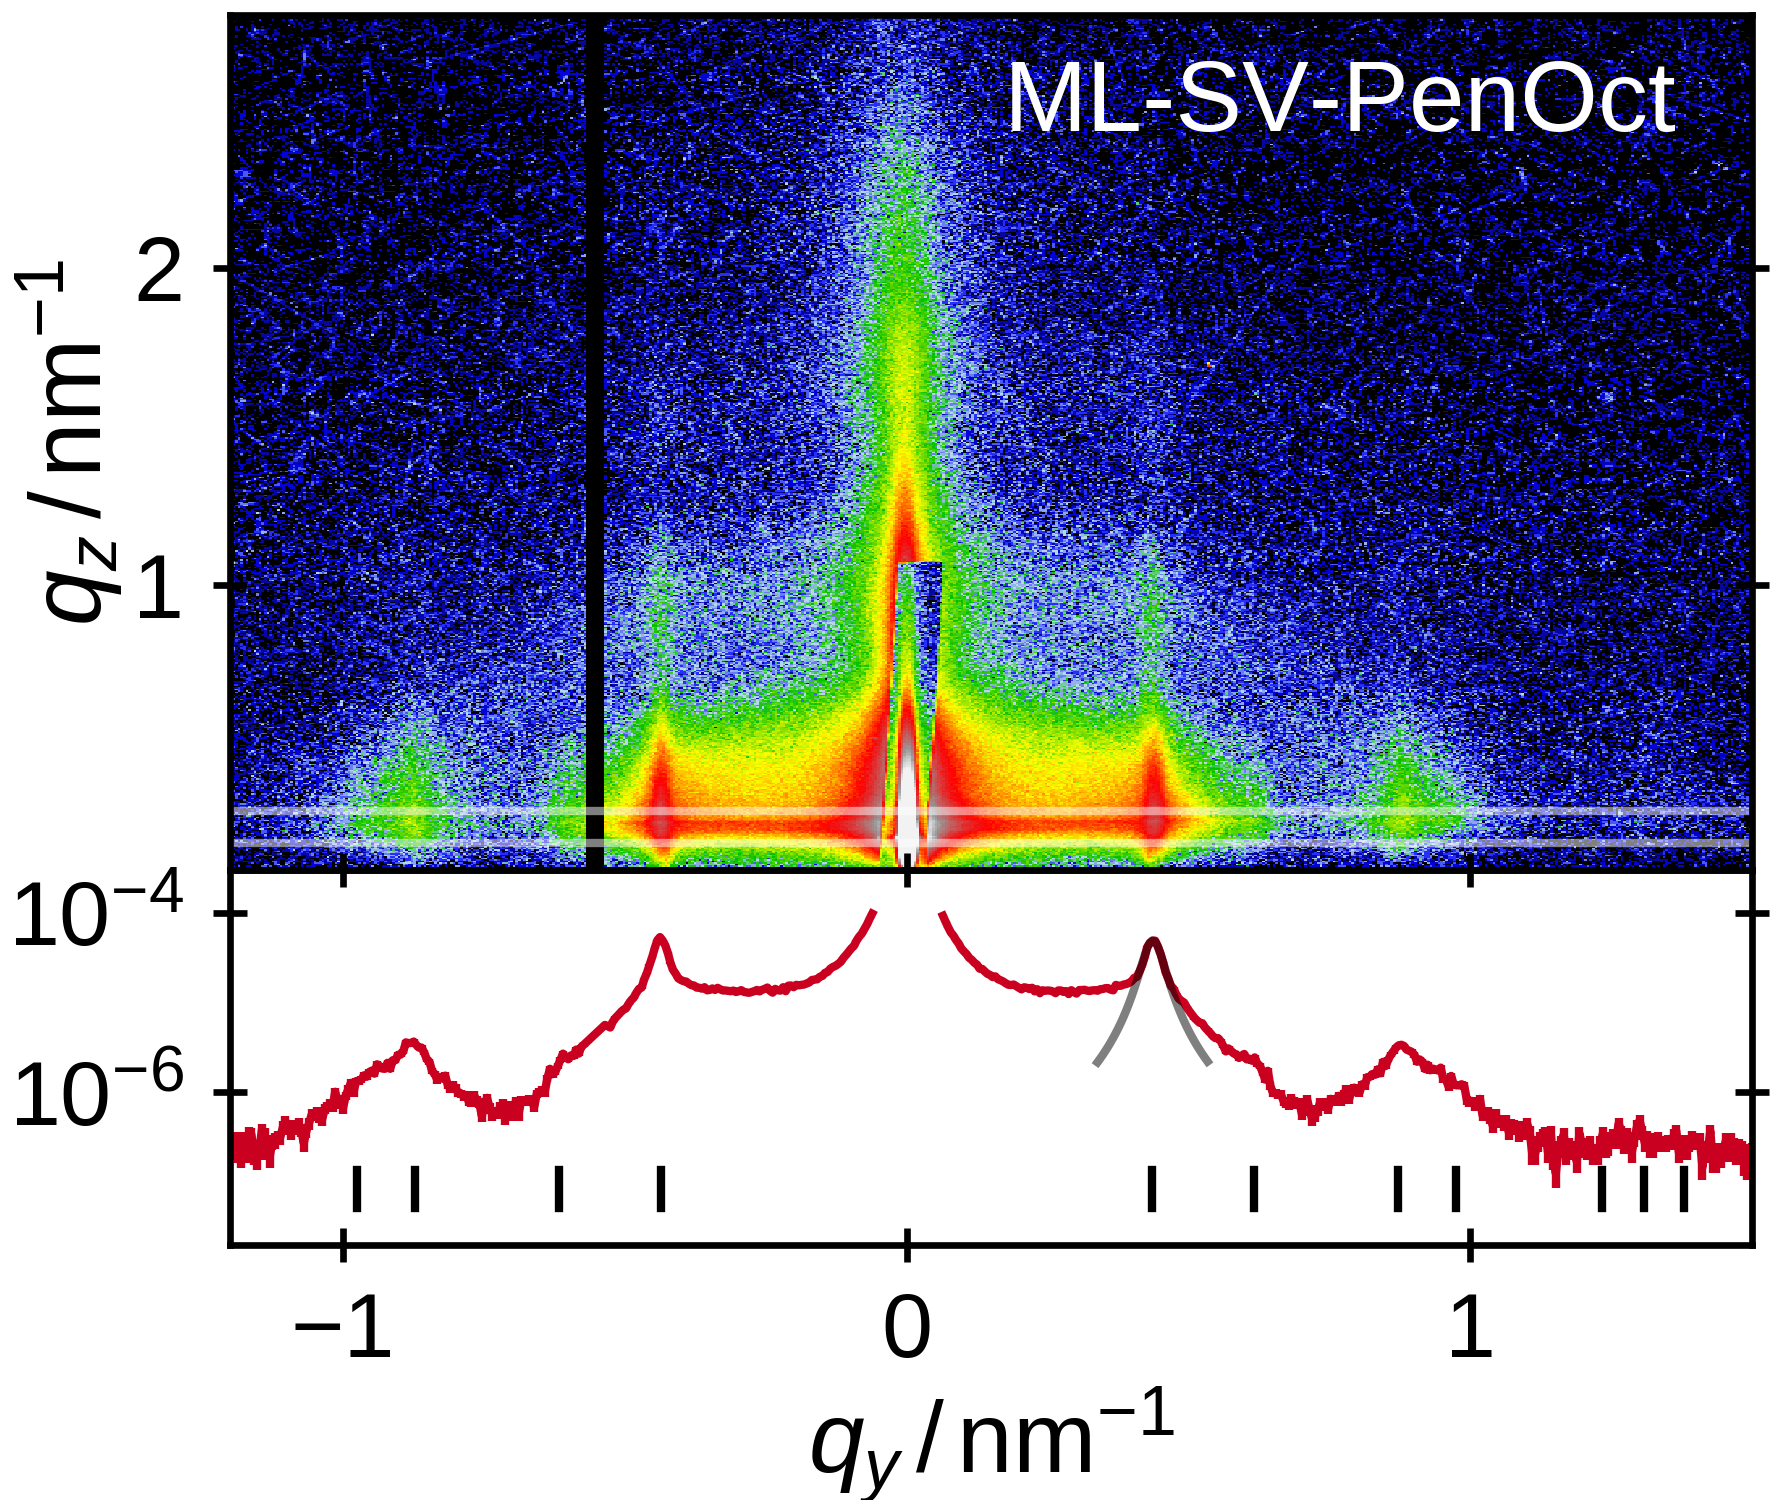
\includegraphics{monolayers_GISAXS_ML-SV-PenOct}
      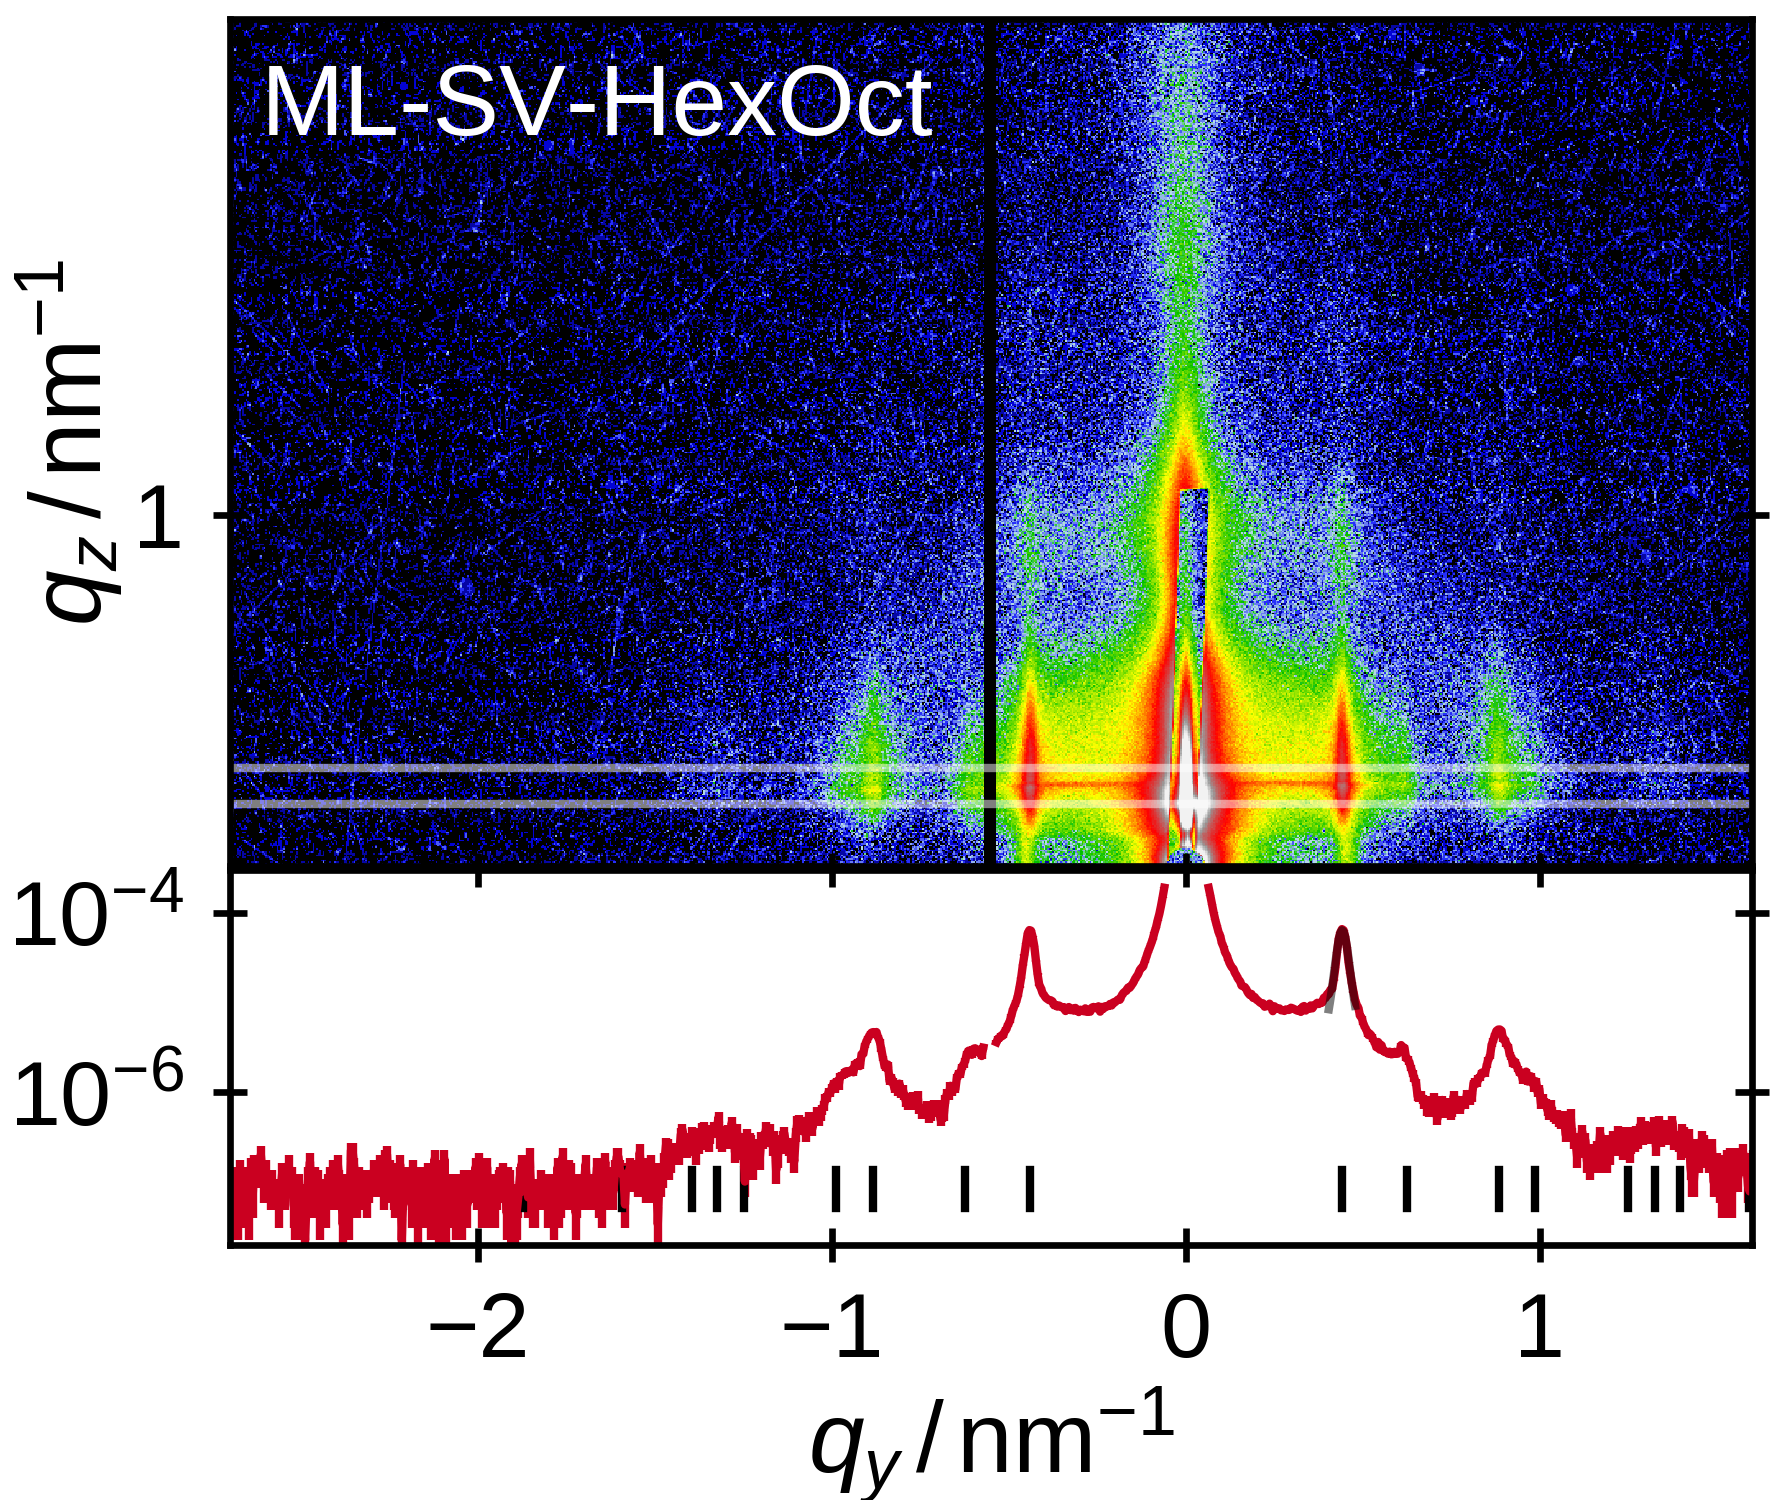
\includegraphics{monolayers_GISAXS_ML-SV-HexOct}
      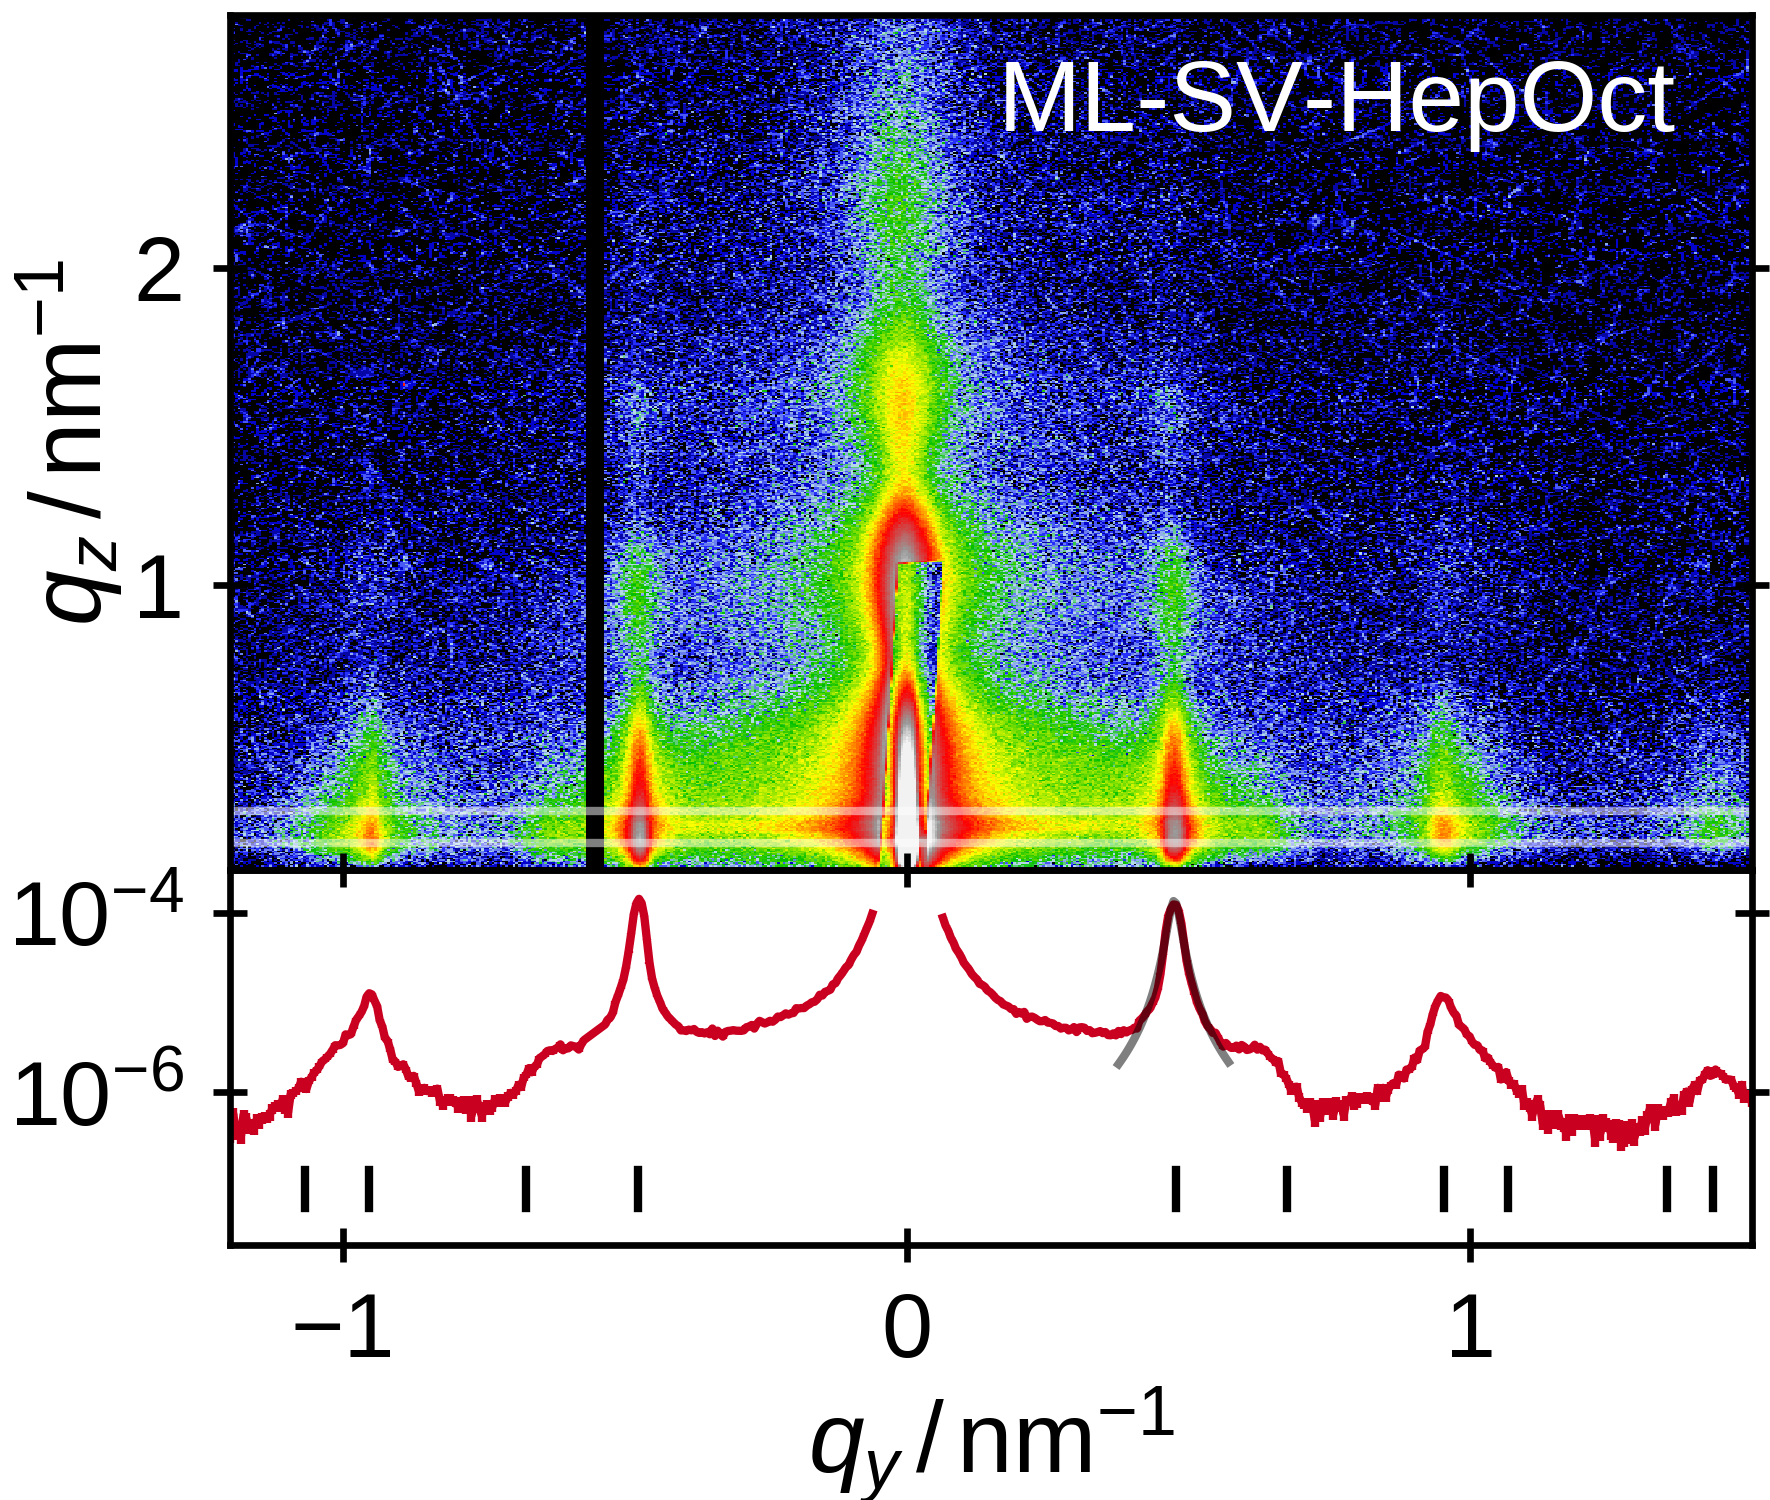
\includegraphics{monolayers_GISAXS_ML-SV-HepOct}
      \caption{\label{fig:monolayers:preparation:solventVariation:gisaxs}GISAXS detector images measured under an incident angle of $\alpha_i \eq 0.11 \unit{^\circ}$ to study the average lateral structure of the samples shown in \reffig{fig:monolayers:preparation:solventVariation:sem}. Below the detector images, the respective scattered intensity in the strip around the Yoneda line is shown. For the ordered samples, the first order peak is fitted to a Lorentzian function with the parameters tabulated in \reftab{tab:monolayers:solventProperties:GisaxsLatticeParams}.}
    \end{figure}

    To quantify the in-plane order, the presented samples are studied using grazing incidence small-angle X-ray scattering at GALAXI (\refch{ch:lss:galaxi}), shown in \reffig{fig:monolayers:preparation:solventVariation:gisaxs}.
    ML-SV-HexTet shows no significant structure factor in the Yoneda band, but mainly scattering coming from the form factor of the individual nanoparticles.
    For the other three shown samples distinct peaks emerge on top, which increase in intensity for higher order alkanes.
    The first order peak of the structured monolayers is fit by a Lorentzian function to determine it's center position  $q_{10}$ and it's peak width $\gamma_{10}$, which both are tabulated in \reftab{tab:monolayers:solventProperties:GisaxsLatticeParams}.
    The expected peak positions for a square array are deduced from $q_{10}$ and shown as black bars below the projected intensity of the Yoneda line.
    For ML-SV-HexOct and ML-SV-HepOct the position of all peaks fit to the square array pattern.
    For ML-SV-PenOct the (11) peak position is only visible as a shoulder, due to the close proximity to a form factor minimum and it's low intensity.

    \begin{table}[tb]
      \centering
      \caption{\label{tab:monolayers:solventProperties:GisaxsLatticeParams}Scattering vector $q_{10}$ and peak width $gammalta q_{10}$ of the first order peak observed in the GISAXS detector images in \reffig{fig:monolayers:preparation:solventVariation:gisaxs}. From the scattering vector, the lattice constant $a$ is determined and from the peak width, the coherence length $L_{\mathrm{coh.}}$ is calculated.}
      \begin{tabular}{ c | l | l || l | l | l}
        \textbf{GISAXS}  & $q_{10} \,/ \unit{nm^{-1}}$ & $\gamma_{10} \, / \unit{nm^{-1}}$ & $a\, / \unit{nm}$ & $L_{\mathrm{coh.}}\, / \unit{nm}$ & $\sigma_\mathrm{n.N.} \, / \unit{nm}$ \\
        \hline
        ML-SV-PenOct    & $0.4367(3)$    & $0.042(1)$    & $14.39(1)$    & $1061(35)$  & $1.()$\\
        ML-SV-HexOct    & $0.4342(1)$    & $0.030(1)$    & $14.22(1)$    & $1721(86)$  & $1.()$\\
        ML-SV-HepOct    & $0.4747(6)$    & $0.024(2)$    & $13.24(2)$    & $2662(477)$ & $1.()$\\
        \hline
      \end{tabular}
    \end{table}

    A close inspection of the peak positions and width in \reftab{tab:monolayers:solventProperties:GisaxsLatticeParams} shows that for increasing order of alkane, the lattice constant reduces and the coherence length increases.
    Both can be explained by an improved packing of the square lattice and tells that higher alkanes increase the long-range order.
  \FloatBarrier
\end{document}